\section{Ransac mit Maskierung}

Aus einem Foto mittels \gls{acr:ransac} eine mathematische Approximation für eine Linie zu erhalten, war die von uns anfangs bevorzugte Herangehensweise. Durch den festen Entschluss, eine Weltkarte aufzubauen, ist der Gedanke naheliegend, deren Information für das nächste Bild zu nutzen. Voraussetzung dafür ist allerdings, dass die Informationen der Karte verlässlich sind.

\subsection{Vorteile}
Ein mathematisches Modell hinter der Linienerkennung bietet einige Vorteile:
\begin{itemize}
\item Im Gegensatz zu einer Geraden, einem Kreis oder einer quadratischen Funktion kann das gewählte Polynom dritten Grades zusätzlich dem Verlauf einer S-Kurve (Übergang einer Links- in eine Rechtskurve und umgekehrt) relativ gut folgen. \item Unter der Annahme einer guten Annäherung zur echten Markierung kann im Falle eines unbrauchbaren Fotos durch Extrapolation trotzdem weitergefahren werden. 
\item Die Stetigkeit der kubischen Funktion verhindert das plötzliche Abknicken des Linienverlaufs, sodass nahezu senkrecht auftreffende Querstraßenmarkierungen nicht als Kurve erkannt werden
\item Durch die Anwendung von \gls{acr:ransac} haben Unterbrechungen oder kleine Störungen keinen negativen Einfluss. Als Outlier erkannte Pixel werden in der anschließenden Regression nicht berücksichtigt.
\end{itemize}

\subsection{Probleme}
Trotz der vielen Vorzüge bringt gerade \gls{acr:ransac} das Problem mit sich, dass in einem Bildausschnitt nur ein Markierungsverlauf gefunden wird. Daher müssen in einer Aufnahme drei sinnvoll gewählte Bereiche feststehen, in welchen je ein \gls{acr:ransac}-Algorithmus ausgeführt werden kann. 
Das größte Problem, welches letztlich zum Ausschluss der \gls{acr:ransac}-Methode geführt hat, ist die zuverlässige Bestimmung dieser \gls{acr:roi}. Wie auch schon in Abb.~\ref{fig:fahrspurerkennung_ransac_ransac} Bild (a) zu sehen war, approximiert das Polynom den Linienverlauf am Bildrand deutlich schlechter. Entgegen der Erwartung sind die Extrapolationseigenschaften von Polynomen zum Maskenbau ungeeignet. Die Funktion steigt am Bildrand meist stärker als die zu erkennende Kurve. Dies führt zu falsch vorhergesagten \glspl{roi}, welche beispielhaft in Abb.~\ref dargestellt sind.

\begin{figure}[H]
	\centering
	\subfloat[][]{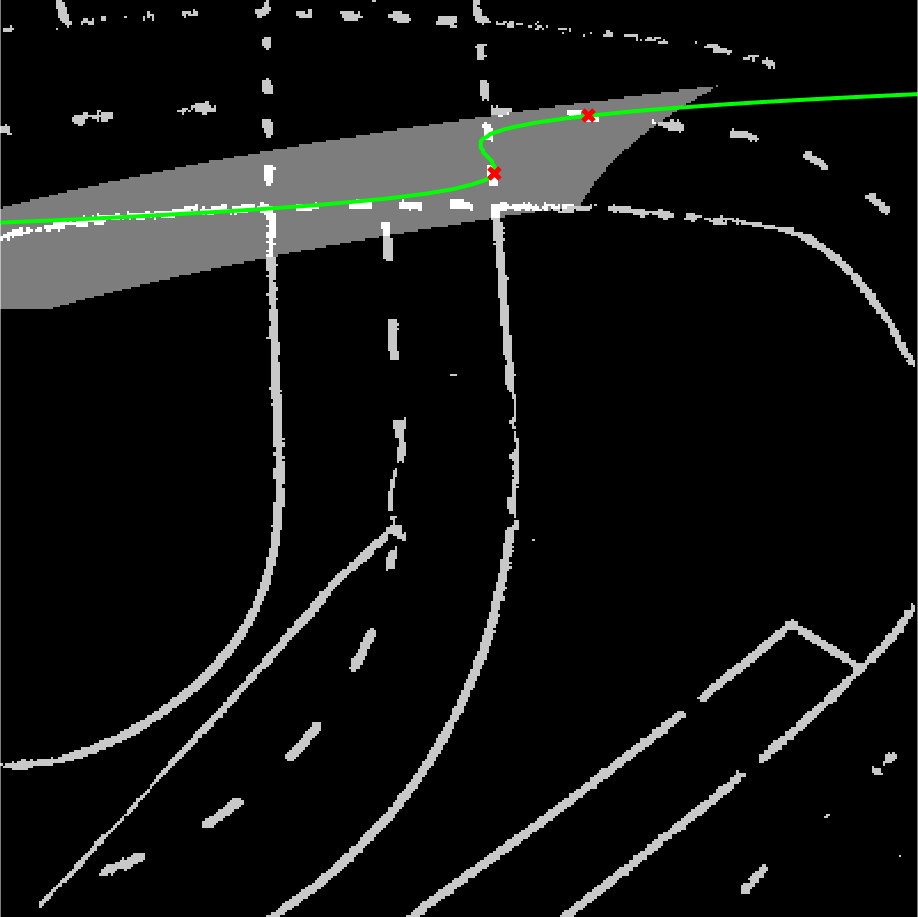
\includegraphics[width=0.3\textwidth]{evaluation_ransac_imgMaskLeft.png}}
	\quad
	\subfloat[][]{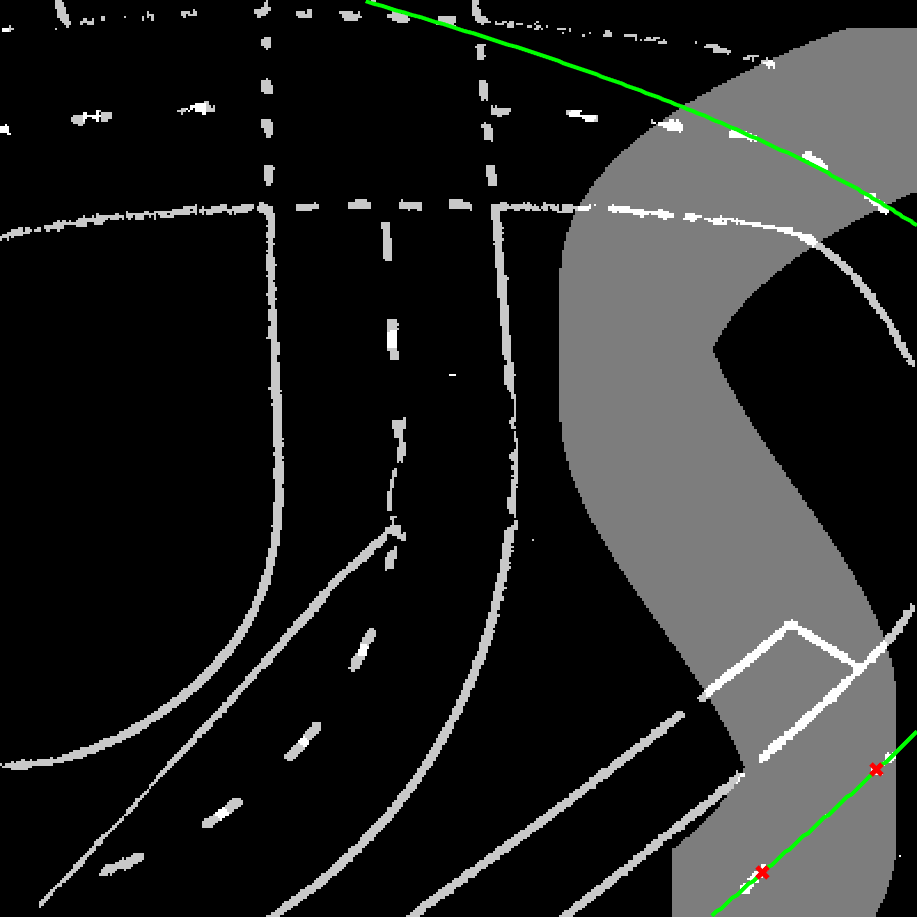
\includegraphics[width=0.3\textwidth]{evaluation_ransac_imgMaskMiddle.png}}
	\quad
	\subfloat[][]{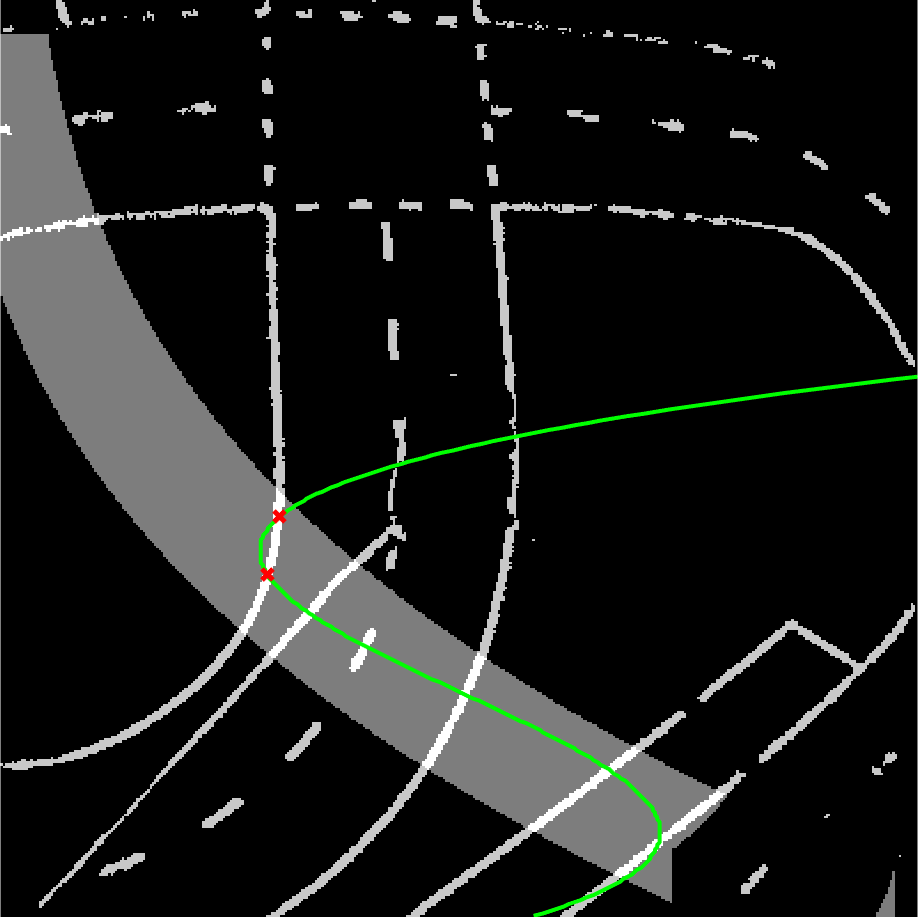
\includegraphics[width=0.3\textwidth]{evaluation_ransac_imgMaskRight.png}}
	\caption{Fehlerhaft erzeugte Masken der linken (a), mittleren (b) und rechten (c) Fahrbahnmarkierungen während eines Testlaufes}
	\label{fig:fahrspurerkennung_ransac_ransac}
\end{figure} 



% Bild/Plot der eingetragenen Punkte in der Weltkarte nach ein paar Sekunden
\begin{figure}[H] % [htb]
  \centering
  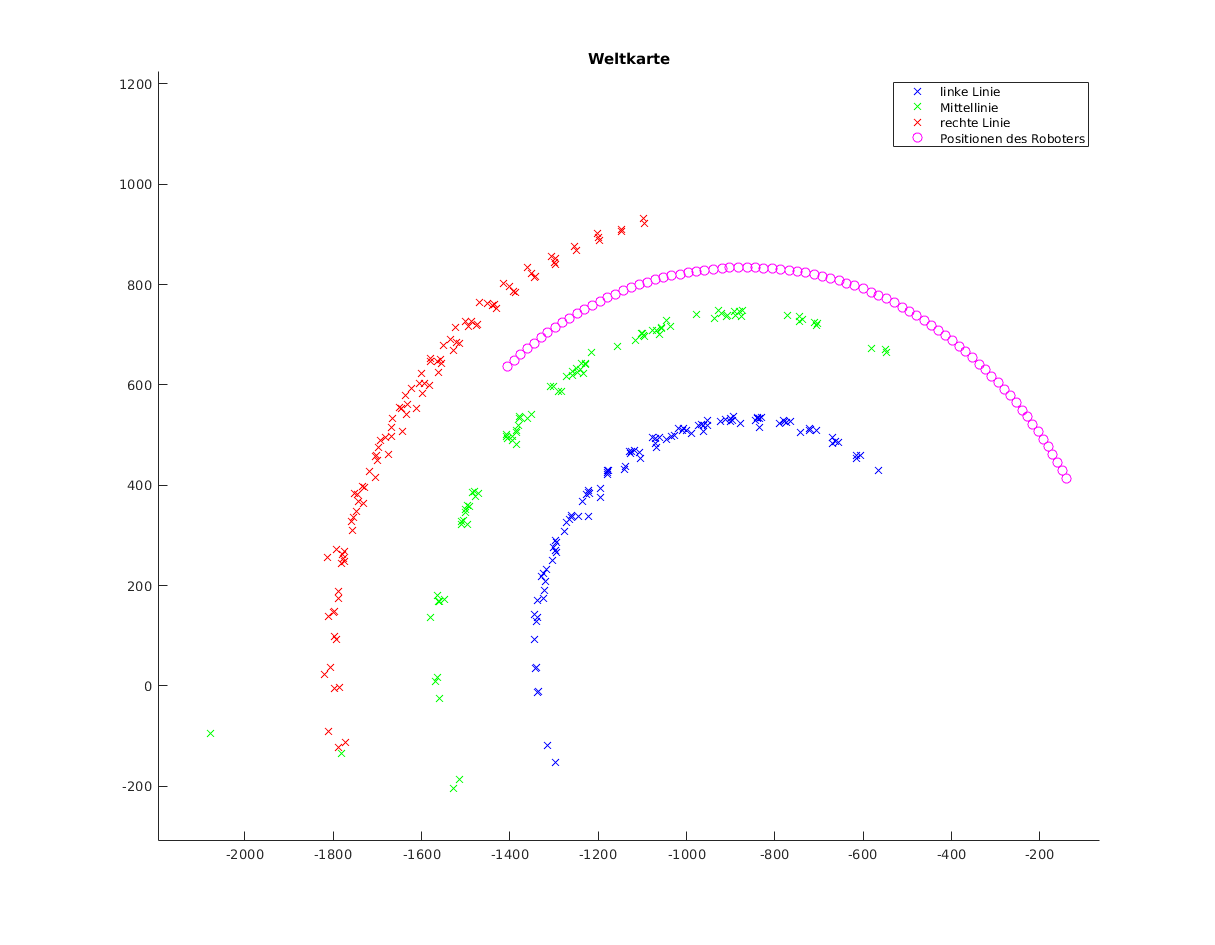
\includegraphics[width=1\textwidth]{evaluation_ransac_erkannte_Kurve.png}
  \caption{Plot der Weltkarte nach kurzer Laufzeit mit einem rosbag-file}
\label{evaluation_ransac_weltkarte_kurve}
\end{figure} 